% begin module transformations-shifts
\begin{frame}
\frametitle{Transformations of Functions}
\begin{columns}[c]
\column{.5\textwidth}
\ \only<handout:0| -2>{%
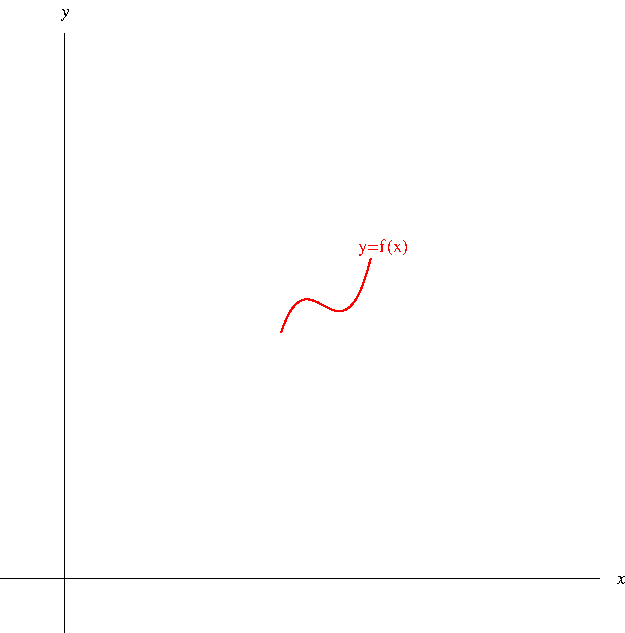
\includegraphics[height=5cm]{precalculus/pictures/01-03-shifta.pdf}%
}%
\only<handout:0| 3>{%
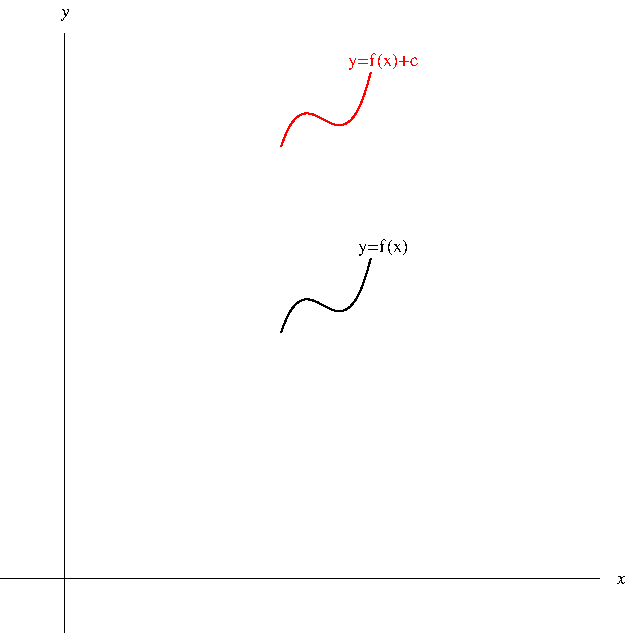
\includegraphics[height=5cm]{precalculus/pictures/01-03-shiftb.pdf}%
}%
\only<handout:0| 4>{%
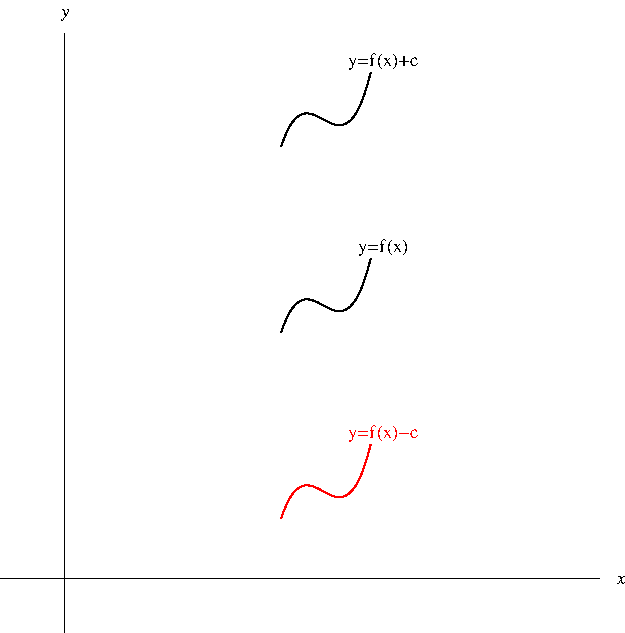
\includegraphics[height=5cm]{precalculus/pictures/01-03-shiftc.pdf}%
}%
\only<handout:0| 5>{%
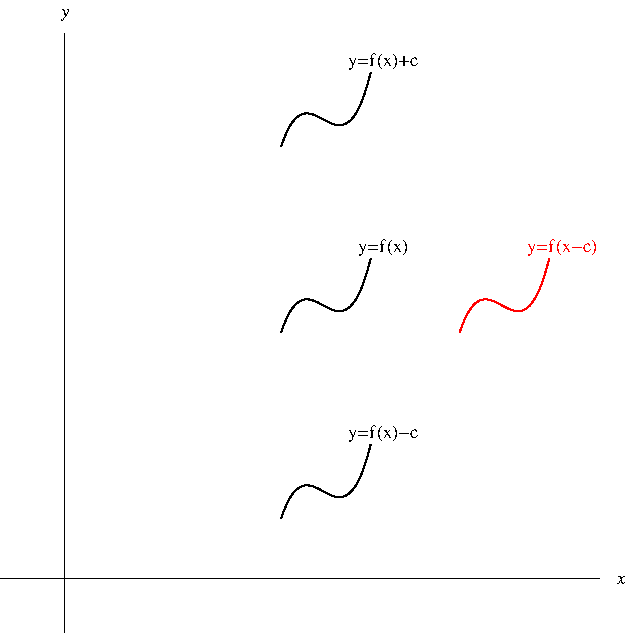
\includegraphics[height=5cm]{precalculus/pictures/01-03-shiftd.pdf}%
}%
\only<6>{%
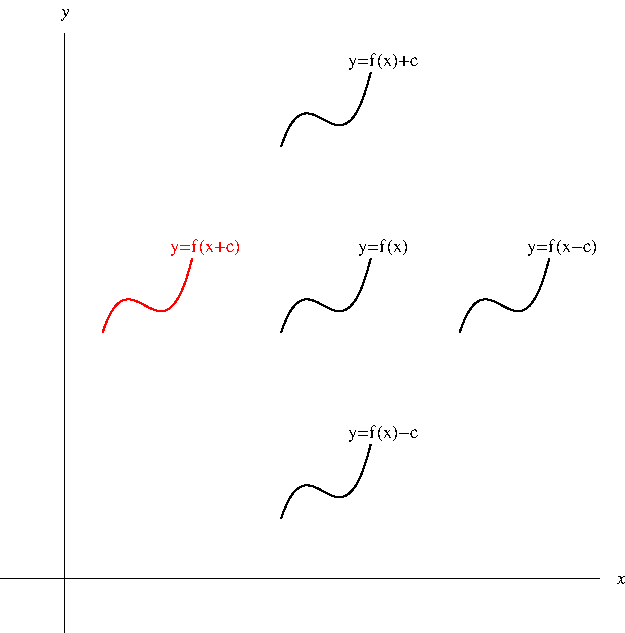
\includegraphics[height=5cm]{precalculus/pictures/01-03-shifte.pdf}%
}%a
\column{.5\textwidth}
What happens if we add or subtract a positive constant $c$ in the equation of a function $f$?  What happens if we add or subtract $c$ from $x$ before applying the function $f$?
\end{columns}

\uncover<2->{
\begin{tabular}{|l|l|}
\hline
\alert<handout:0| 3>{$f(x)+c$} &%
\uncover<3->{\alert<handout:0| 3>{Shift the graph of $f(x)$ $c$ units up.}} \\%
\alert<handout:0| 4>{$f(x)-c$} &%
\uncover<4->{\alert<handout:0| 4>{Shift the graph of $f(x)$ $c$ units down.}} \\%
\alert<handout:0| 5>{$f(x-c)$} &%
\uncover<5->{\alert<handout:0| 5>{Shift the graph of $f(x)$ $c$ units right.}} \\%
\alert<handout:0| 6>{$f(x+c)$} &%
\uncover<6->{\alert<handout:0| 6>{Shift the graph of $f(x)$ $c$ units left.}}\\%
\hline
\end{tabular}
}
\end{frame}
% end module transformations-shifts
